%package list
\documentclass{article}
\usepackage[top=3cm, bottom=3cm, outer=3cm, inner=3cm]{geometry}
\usepackage{multicol}
\usepackage{graphicx}
\usepackage{url}
%\usepackage{cite}
\usepackage{hyperref}
\usepackage{array}
%\usepackage{multicol}
\newcolumntype{x}[1]{>{\centering\arraybackslash\hspace{0pt}}p{#1}}
\usepackage{natbib}
\usepackage{pdfpages}
\usepackage{multirow}
\usepackage[normalem]{ulem}
\useunder{\uline}{\ul}{}
\usepackage{svg}
\usepackage{xcolor}
\usepackage{listings}
\lstdefinestyle{ascii-tree}{
    literate={├}{|}1 {─}{--}1 {└}{+}1 
  }
\lstset{basicstyle=\ttfamily,
  showstringspaces=false,
  commentstyle=\color{red},
  keywordstyle=\color{blue}
}
%\usepackage{booktabs}
\usepackage{caption}
\usepackage{subcaption}
\usepackage{float}
\usepackage{array}

\newcolumntype{M}[1]{>{\centering\arraybackslash}m{#1}}
\newcolumntype{N}{@{}m{0pt}@{}}


%%%%%%%%%%%%%%%%%%%%%%%%%%%%%%%%%%%%%%%%%%%%%%%%%%%%%%%%%%%%%%%%%%%%%%%%%%%%
%%%%%%%%%%%%%%%%%%%%%%%%%%%%%%%%%%%%%%%%%%%%%%%%%%%%%%%%%%%%%%%%%%%%%%%%%%%%
\newcommand{\itemEmail}{jperez@unsa.edu.pe}
\newcommand{\itemStudent}{Juan Perez Luna}
\newcommand{\itemCourse}{Programación}
\newcommand{\itemCourseCode}{1702122}
\newcommand{\itemSemester}{III}
\newcommand{\itemUniversity}{Universidad Nacional de San Agustín de Arequipa}
\newcommand{\itemFaculty}{Facultad de Ingeniería de Producción y Servicios}
\newcommand{\itemDepartment}{Departamento Académico de Ingeniería de Sistemas e Informática}
\newcommand{\itemSchool}{Escuela Profesional de Ingeniería de Sistemas}
\newcommand{\itemAcademic}{2023 - A}
\newcommand{\itemInput}{Del 26 Junio 2023}
\newcommand{\itemOutput}{Al 03 Julio 2023}
\newcommand{\itemPracticeNumber}{07}
\newcommand{\itemTheme}{Django Rest Framework}
%%%%%%%%%%%%%%%%%%%%%%%%%%%%%%%%%%%%%%%%%%%%%%%%%%%%%%%%%%%%%%%%%%%%%%%%%%%%
%%%%%%%%%%%%%%%%%%%%%%%%%%%%%%%%%%%%%%%%%%%%%%%%%%%%%%%%%%%%%%%%%%%%%%%%%%%%

\usepackage[english,spanish]{babel}
\usepackage[utf8]{inputenc}
\AtBeginDocument{\selectlanguage{spanish}}
\renewcommand{\figurename}{Figura}
\renewcommand{\refname}{Referencias}
\renewcommand{\tablename}{Tabla} %esto no funciona cuando se usa babel
\AtBeginDocument{%
	\renewcommand\tablename{Tabla}
}

\usepackage{fancyhdr}
\pagestyle{fancy}
\fancyhf{}
\setlength{\headheight}{30pt}
\renewcommand{\headrulewidth}{1pt}
\renewcommand{\footrulewidth}{1pt}
\fancyhead[L]{\raisebox{-0.2\height}{
\includegraphics[width=3cm]{img/logo_episunsa.png}}}
\fancyhead[C]{\fontsize{7}{7}\selectfont	\itemUniversity \\ \itemFaculty \\ \itemDepartment \\ \itemSchool \\ \textbf{\itemCourse}}
\fancyhead[R]{\raisebox{-0.2\height}{
\includegraphics[width=1.2cm]{img/logo_abet}}}
\fancyfoot[L]{Estudiante Juan Perez Perez}
\fancyfoot[C]{\itemCourse}
\fancyfoot[R]{Página \thepage}

% para el codigo fuente
\usepackage{listings}
\usepackage{color, colortbl}
\definecolor{dkgreen}{rgb}{0,0.6,0}
\definecolor{gray}{rgb}{0.5,0.5,0.5}
\definecolor{mauve}{rgb}{0.58,0,0.82}
\definecolor{codebackground}{rgb}{0.95, 0.95, 0.92}
\definecolor{tablebackground}{rgb}{0.8, 0, 0}

\lstset{frame=tb,
	language=bash,
	aboveskip=3mm,
	belowskip=3mm,
	showstringspaces=false,
	columns=flexible,
	basicstyle={\small\ttfamily},
	numbers=none,
	numberstyle=\tiny\color{gray},
	keywordstyle=\color{blue},
	commentstyle=\color{dkgreen},
	stringstyle=\color{mauve},
	breaklines=true,
	breakatwhitespace=true,
	tabsize=3,
	backgroundcolor= \color{codebackground},
}

\begin{document}
	
	\vspace*{10px}
	
	\begin{center}	
		\fontsize{17}{17} \textbf{ Informe de Laboratorio \itemPracticeNumber}
	\end{center}
	\centerline{\textbf{\Large Tema: \itemTheme}}
	%\vspace*{0.5cm}	

	\begin{flushright}
		\begin{tabular}{|M{2.5cm}|N|}
			\hline 
			\rowcolor{tablebackground}
			\color{white} \textbf{Nota}  \\
			\hline 
			     \\[30pt]
			\hline 			
		\end{tabular}
	\end{flushright}	

	\begin{table}[H]
		\begin{tabular}{|x{4.7cm}|x{4.8cm}|x{4.8cm}|}
			\hline 
			\rowcolor{tablebackground}
			\color{white} \textbf{Estudiante} & \color{white}\textbf{Escuela}  & \color{white}\textbf{Asignatura}   \\
			\hline 
			{Hidalgo Chinchay, Paulo Andre \par phidalgo@unsa.edu.pe \par Huayhua Mayta, Iván Rodrigo \par ihuayhuam@unsa.edu.pe \par Jaita Chura, José Manuel \par jjaitac@unsa.edu.pe \par Garcia Valdivia, Ronald Pablo\par rgarciava@unsa.edu.pe} & \itemSchool & {\itemCourse \par Semestre: \itemSemester \par Código: \itemCourseCode}     \\
			\hline 			
		\end{tabular}
	\end{table}		
	
	\begin{table}[H]
		\begin{tabular}{|x{4.7cm}|x{4.8cm}|x{4.8cm}|}
			\hline 
			\rowcolor{tablebackground}
			\color{white}\textbf{Laboratorio} & \color{white}\textbf{Tema}  & \color{white}\textbf{Duración}   \\
			\hline 
			\itemPracticeNumber & \itemTheme & 04 horas   \\
			\hline 
		\end{tabular}
	\end{table}
	
	\begin{table}[H]
		\begin{tabular}{|x{4.7cm}|x{4.8cm}|x{4.8cm}|}
			\hline 
			\rowcolor{tablebackground}
			\color{white}\textbf{Semestre académico} & \color{white}\textbf{Fecha de inicio}  & \color{white}\textbf{Fecha de entrega}   \\
			\hline 
			\itemAcademic & \itemInput &  \itemOutput  \\
			\hline 
		\end{tabular}
	\end{table}
	
	\section{Competencias del curso}
	\begin{itemize}		
		\item General: C.c. Diseña responsablemente aplicaciones web, sus componentes o procesos para satisfacer necesidades dentro de restricciones realistas: económicas, medio ambientales, sociales, políticas, éticas, de salud, de seguridad, manufacturación y sostenibilidad.
		\item Específica: C.m. Construye responsablemente soluciones con tecnología web siguiendo un pro-
            ceso adecuado llevando a cabo las pruebas ajustada a los recursos disponibles del cliente.
		\item Específica: C.p. Aplica de forma flexible técnicas, métodos, principios, normas, estándares y
            herramientas del desarrollo web necesarias para la construcción de aplicaciones web e implemen-
            tación de estos sistemas en una organización.
	\end{itemize}
 
    \section{Resultado del estudiante}
    \begin{itemize}
        \item RE. 2 La capacidad de aplicar diseño de ingeniería para producir soluciones a problemas y diseñar
            sistemas, componentes o procesos para satisfacer necesidades específicas dentro de consideracio-
            nes realistas en los aspectos de salud pública, seguridad y bienestar; factores globales, culturales,
            sociales, económicos y ambientales.
        \item RE. 8 La capacidad de crear, seleccionar y utilizar técnicas, habilidades, recursos y herramientas
            modernas de ingeniería y tecnologías de la información, incluyendo la predicción y el modela-
            miento, con una comprensión de las limitaciones.
    \end{itemize}
		
	\section{Equipos, materiales y temas}
	\begin{itemize}
		\item Sistema Operativo (GNU/Linux de preferencia).
		\item GNU Vim.
		\item Python 3.
		\item Git.
		\item Cuenta en GitHub con el correo institucional.
		\item Entorno virtual.
		\item Django 4.	
        \item djangorestframework.
	\end{itemize}
	
	\section{URL de Repositorio Github}
	\begin{itemize}
		\item URL del Repositorio GitHub para clonar o recuperar.
		\item \url{https://github.com/123ihuayhua/pweb2-lab-c-23a.git}
		\item URL para el laboratorio 07 en el Repositorio GitHub.
		\item \url{https://github.com/123ihuayhua/pweb2-lab-c-23a/tree/main/Lab7-Pweb2}
	\end{itemize}
    \section{Admin, user y tokens}
    \begin{itemize}
        \item Admin:
        \begin{itemize}
            \item Usuario: admin
            \item Contraseña: 12345
            \item Token: eeef53ad0f9a274f2d2f27426410abb4fe3fb855
        \end{itemize}
        \item User:
        \begin{itemize}
            \item Usuario: Alfonso\_M
            \item Contraseña: alfonso
            \item Token: 8aff82557e15d93fe60bfacf6f86fa9ae34fc3c8
        \end{itemize}
    \end{itemize}

    
    \section{Tarea}
    \begin{itemize}
        \item En sus grupos de trabajo correspondientes. Elabore un servicio web que tenga un CRUD con el uso de este framework.
        \item Create - POST
        \item Read - GET
        \item Update - PUT
        \item Delete - DELETE
        \item Centrarce en el Core business de su aplicación web. Los más importante y necesario que este disponible a traves de un servicio web.
        \item Ejemplos: https://reqbin.com/,https://www.googleapis.com/youtube/v3/playlistItems
        \item Muestre la funcionalidad consumiendola desde el cliente Rest de su preferencia.
        \item El método GET puede ser directamente consumido por un navegador web:
        \item Por ejemplo: En esta API se puede obtener la temperatura de Arequipa en un rango de fechas: (La versión gratuita tiene un retraso de 7 días, por tanto sólo mostrará la temperatura en Arequipa desde el 01 de Julio hasta el 03 de Julio)
        \item https://archive-api.open-meteo.com/v1/archive?latitude=-16.39889\&longitude=-71.535\&start\_date=2023-07-01\&end\_date=2023-07-10\&hourly=temperature\_2m\&daily=temperature\_2m\_max,temperature\_2m\_min\&timezone=America\%2FNew\_York
    \end{itemize}

    \section{Pregunta}
    \begin{itemize}
        \item ¿Cuál fué la mayor dificultad del uso de este framework?.
        \begin{itemize}
            \item Manejo de errores y excepciones: Es importante manejar correctamente los errores y excepciones en una API REST para proporcionar respuestas adecuadas a los usuarios o clientes de la API. (Huayhua Mayta, Iván Rodrigo)
            \item Validación y autenticación: La validación y autenticación de las solicitudes y respuestas pueden ser desafiantes, especialmente cuando se trata de lidiar con diferentes niveles de permisos y roles de usuario. (Garcia Valdivia, Ronald Pablo)
            \item Integración con otras aplicaciones: Al integrar Django REST Framework con otras aplicaciones y módulos, pueden surgir problemas de compatibilidad o conflictos con otras bibliotecas o extensiones utilizadas en el proyecto. (Jaita Chura, José Manuel)
            \item Configuración compleja: Si bien DRF es poderoso y versátil, puede ser complicado configurar y personalizar, especialmente cuando se necesita una funcionalidad específica o características avanzadas. (Hidalgo Chinchay, Paulo Andre)
        \end{itemize}
    \end{itemize}
    
    \section{Entregable}
    \begin{itemize}
        \item El informe debe tener un enlace al directorio específico del laboratorio en su repositorio GitHub
        privado donde esté todo el código fuente y otros que sean necesarios. Evitar la presencia de archi-
        vos: binarios, objetos, archivos temporales, cache, librerias, entornos virtuales. Si hay configura-
        ciones particulares puede incluir archivos de especificación como: requirements.txt, o leeme.txt.
        \item No olvide que el profesor debe ser siempre colaborador a su repositorio (Usuario del profesor
        @rescobedoq).
        \item Para ser considerado con la calificación de máxima nota, el informe debe estar elaborado en
        LATEX
        \item Usted debe describir sólo los commits más importantes que marcaron hitos en su trabajo,
        adjutando capturas de pantalla, del commit, del código fuente, de sus ejecuciones y pruebas.
        \item En el informe siempre se debe explicar las imágenes (codigo fuente, capturas de pantalla, commits,
        ejecuciones, pruebas, etc.) con descripciones puntuales pero precisas.
        \item Partes de entrega:
        \begin{itemize}
            \item Django orientado a Usuarios finales
            \item Tema para clientes, con funcionalidades importantes.
            \item Recomendaciones: CRUD en uno de los procesos para el cliente final
            \item Ejemplo 1: Para la WebApp Library (Sistema de Biblioteca virtual), ser´ıa .El cliente reserva un ejemplar de un libro determinado”.
            \item Ejemplo 2: Para la WebApp Enrollments (Sistema para Inscripciones en laboratorios), sería. El alumno se inscribe en un laboratorio disponible para un curso”.

        \end{itemize}
    \end{itemize}
    \begin{itemize}
        \item carrito.html:
        \item {\% extends 'base.html' \%}: Indica que esta plantilla hereda del archivo 'base.html'. Esto significa que la plantilla actual se extiende a partir de otra plantilla base, que contiene la estructura y el diseño común de todas las páginas del sitio.
        \item : Carga el contexto "static" para poder utilizar los archivos estáticos (como hojas de estilo CSS o archivos JavaScript) en la plantilla.
        \item  y : Estos bloques son marcadores que permiten que el contenido específico de esta plantilla se inserte dentro de un bloque con el mismo nombre en la plantilla base.
        \item <link rel="stylesheet" href="https://cdn.jsdelivr.net/npm/sweetalert2@11.1.4/dist/sweetalert2.min.css">: Se carga la hoja de estilos de la librería Swal (SweetAlert2), que se utiliza para mostrar alertas y mensajes emergentes.
        \item <div class="banner">...</div>: Aquí se muestra un banner con una imagen y un título "Carrito de Compras". La imagen del banner se obtiene de la carpeta de archivos estáticos usando la etiqueta {\% static \%}.
        \item <div>...</div>: Esta parte muestra mensajes de alerta (en caso de que haya) utilizando el framework de mensajes de Django.
        \item <div class="container">...</div>: Aquí se muestra el contenido principal del carrito de compras. Si el carrito no está vacío (es decir, si hay elementos en el carrito), se muestra una tabla con los detalles de los productos en el carrito. Cada fila de la tabla contiene el nombre del producto, la cantidad, el precio unitario, el subtotal y un botón para eliminar el producto del carrito. Además, se muestra el total del carrito al final de la tabla. Los botones de la tabla llaman a funciones JavaScript (sumarCantidad, restarCantidad, actualizarCantidad y eliminarProducto) para actualizar la cantidad de productos en el carrito.
        \item <script>...</script>: Este bloque contiene código JavaScript que define funciones utilizadas para gestionar la cantidad de productos en el carrito, eliminar productos, guardar el pedido y cancelar el carrito. También se utiliza la librería Swal para mostrar mensajes emergentes de confirmación y notificación.
        \item En resumen, esta plantilla HTML muestra el contenido del carrito de compras de una aplicación web, permite al usuario interactuar con los elementos del carrito (agregar o disminuir la cantidad de productos, eliminar productos) y realizar acciones como guardar el pedido o cancelar el carrito, todo ello utilizando JavaScript y alertas visuales a través de SweetAlert2. Además, extiende de una plantilla base, lo que le da una estructura y diseño común en toda la aplicación.
    \end{itemize}
    \lstinputlisting[language=Python, caption={carrito.html},numbers=left,]{src/carrito.html}
    \begin{itemize}
        \item pedido\_detalle.html.
        \item En el bloque de contenido, se define una estructura con contenedores para mostrar los datos del pedido.
        \item La primera parte muestra el encabezado "DATOS DEL PEDIDO" y presenta una tabla con detalles como el cliente, la fecha y el total del pedido.
        \item La segunda parte muestra una tabla con los detalles de los artículos del pedido (detalles del pedido). Utiliza un bucle {\% for detalle in detalles \%} para iterar sobre cada detalle del pedido.
        \item Dentro del bucle, se muestra la información de cada detalle del pedido, incluyendo el artículo, la cantidad, el precio unitario y el subtotal.
        \item Para mostrar los valores de cada detalle del pedido, se utilizan etiquetas de interpolación de Django, como {{ pedido.PedCabCodCli }} y {{ detalle.PedDetArtCod }}, que acceden a los campos de los modelos relacionados.
        \item En resumen, esta plantilla se utiliza para mostrar los detalles de un pedido específico en una página web. Los datos del pedido se presentan en una tabla con información como el cliente, la fecha, el total y los detalles de los artículos del pedido.
    \end{itemize}
    \lstinputlisting[language=Python, caption={pedido_detalle.html},numbers=left,]{src/pedido_detalle.html}
    
    \begin{itemize}
        \item A continuación se detalla la función de cada parte del código api.py:
        \item VendedorViewSet: Permite realizar operaciones CRUD (Crear, Leer, Actualizar, Eliminar) en el modelo Vendedor. Está configurado para que solo los usuarios administradores puedan realizar todas las operaciones, mientras que los usuarios autenticados pueden leer los datos (operaciones de solo lectura) y los usuarios no autenticados pueden acceder solo para lectura (operaciones de solo lectura).
        \item ClienteViewSet: Similar al VendedorViewSet, pero este maneja el modelo Cliente y solo permite que los usuarios administradores realicen operaciones CRUD.
        \item MarcaViewSet: Similar a los anteriores, pero se enfoca en el modelo Marca y permite que los usuarios administradores realicen todas las operaciones CRUD, mientras que los usuarios autenticados pueden realizar solo operaciones de lectura.
        \item TipoArticuloViewSet: Igual que los anteriores, pero maneja el modelo TipoArticulo.
        \item ArticuloViewSet: Permite operaciones CRUD en el modelo Articulo, al igual que los otros ViewSets, restringiendo algunas operaciones a los usuarios administradores y permitiendo que los usuarios autenticados realicen operaciones de lectura.
        \item PedidoViewSet: Similar a los anteriores, pero para el modelo Pedido, permitiendo que los usuarios administradores realicen todas las operaciones CRUD y que los usuarios autenticados solo realicen operaciones de lectura.
        \item CarritoViewSet: Permite a los usuarios autenticados realizar operaciones CRUD en el modelo Carrito.
        \item PedidoView (APIView):
        \begin{itemize}
            \item post: Esta vista permite crear un nuevo objeto Pedido utilizando el serializador PedidoSerializer y los datos proporcionados en el cuerpo de la solicitud POST. Luego devuelve los datos del pedido creado con el estado HTTP 201 Created.
            \item delete: Esta vista permite eliminar un objeto Pedido específico mediante una solicitud DELETE con el ID del pedido a eliminar (pk). Después de eliminar el pedido, devuelve una respuesta con el estado HTTP 204 No Content.
        \end{itemize}
        \item Este además nos define quieres pueden ver los datos como re artículos, clientes y vendedores.
    \end{itemize}
    \lstinputlisting[language=Python, caption={api.py},numbers=left,]{src/api.py}

    \begin{itemize}
        \item La funcionalidad de models.py es la siguiente:
        \item Vendedor: Representa un vendedor en la aplicación. Tiene campos como VenDNI (documento de identidad), VenApePat (apellido paterno), VenNom (nombre), y VenEstReg (estado de registro). El método \_\_str\_\_ devuelve el nombre completo del vendedor.
        \item Cliente: Hereda de AbstractUser, lo que significa que es un modelo de usuario personalizado. Tiene campos adicionales como CliDNI (documento de identidad), CliApePat (apellido paterno), CliNom (nombre), y CliEstReg (estado de registro). También tiene los campos password y username, pero se definen como campos adicionales en lugar de utilizar los campos ya existentes de AbstractUser. El método \_\_str\_\_ devuelve el nombre completo del cliente. Además, se define el método generate\_auth\_token, que crea un token de autenticación asociado al cliente.
        \item Marca: Representa una marca en la aplicación. Tiene campos como MarNom (nombre de la marca), MarImg (imagen de la marca), y MarEstReg (estado de registro). El método \_\_str\_\_ devuelve el nombre de la marca.
        \item TipoArticulo: Representa un tipo de artículo en la aplicación. Tiene campos como TipArtNom (nombre del tipo de artículo) y TipArtEstReg (estado de registro). El método \_\_str\_\_ devuelve el nombre del tipo de artículo.
        \item Articulo: Representa un artículo en la aplicación. Tiene campos como ArtMarCod (clave externa que vincula el artículo con una marca), ArtTipCod (clave externa que vincula el artículo con un tipo de artículo), ArtNom (nombre del artículo), ArtDes (descripción del artículo), ArtImg (imagen del artículo), ArtSto (stock disponible), ArtPreUni (precio unitario), y ArtEstReg (estado de registro). Los métodos \_\_str\_\_, disminuir\_stock y aumentar\_stock se utilizan para obtener una representación de texto del artículo y actualizar el stock del mismo.
        \item Pedido: Representa un pedido realizado por un cliente. Tiene campos como PedCabCodCli (clave externa que vincula el pedido con un cliente), PedCabFec (fecha del pedido, se establece automáticamente al crear el pedido), PedDetArtCod (clave externa que vincula el pedido con un artículo), PedDetCantidad (cantidad del artículo en el pedido), PedDetPreUniArt (precio unitario del artículo en el momento del pedido), PedDetSubtotal (subtotal del artículo en el pedido), PedDetTot (total del pedido), y PedDetEstReg (estado de registro). El método save se utiliza para calcular el subtotal y el total del pedido y actualizar el precio unitario. También se definen los métodos \_\_str\_\_, total, y eliminar para obtener una representación de texto del pedido, calcular el total del pedido y eliminar el pedido.
        \item Carrito: Representa el carrito de compras de un cliente. Tiene campos como usuario (clave externa que vincula el carrito con un cliente), articulo (clave externa que vincula el carrito con un artículo), cantidad (cantidad del artículo en el carrito), y pedido (clave externa que vincula el carrito con un pedido, si el artículo se ha comprado). Los métodos \_\_str\_\_, subtotal, y total se utilizan para obtener una representación de texto del carrito, calcular el subtotal y el total del artículo en el carrito.
        \item En resumen, este código define los modelos y métodos necesarios para implementar una aplicación web que maneja vendedores, clientes, marcas, tipos de artículos, artículos, pedidos y carritos de compras, y realiza algunas funcionalidades adicionales, como el cálculo del total y el subtotal de los pedidos y carritos. También proporciona un método para generar tokens de autenticación para los clientes.
        
    \end{itemize}
    
    \lstinputlisting[language=Python, caption={models.py},numbers=left,]{src/models.py}

    \begin{itemize}
        \item A continuación, se explican brevemente los serializadores definidos en serializers.py:
        \item VendedorSerializer: Se utiliza para serializar y deserializar objetos del modelo Vendedor. Los campos que se incluirán en la representación JSON del vendedor son id, VenDNI, VenApePat, VenNom, y VenEstReg.
        \item ClienteSerializer: Similar al VendedorSerializer, pero se utiliza para el modelo Cliente. Además de los campos id, CliDNI, CliApePat, CliNom, y CliEstReg, también incluye los campos password y username, pero estos campos no serán actualizables en la serialización (operaciones de solo lectura).
        \item MarcaSerializer: Se utiliza para el modelo Marca y serializa los campos id, MarNom, MarImg, y MarEstReg.
        \item TipoArticuloSerializer: Similar a los anteriores, pero para el modelo TipoArticulo. Serializa los campos id, TipArtNom, y TipArtEstReg.
        \item ArticuloSerializer: Se utiliza para el modelo Articulo. Serializa los campos id, ArtMarCod, ArtTipCod, ArtNom, ArtDes, ArtImg, ArtSto, ArtPreUni, y ArtEstReg.
        \item PedidoSerializer: Se utiliza para el modelo Pedido. Serializa los campos id, PedCabCodCli, PedCabFec, PedDetArtCod, PedDetCantidad, PedDetPreUniArt, PedDetSubtotal, PedDetTot, y PedDetEstReg. El campo PedCabFec es de solo lectura y se establece automáticamente al crear el pedido. Además, contiene un método personalizado create\_pedido que permite crear un nuevo pedido y realizar ciertas operaciones relacionadas con el cálculo del subtotal y la disminución del stock del artículo correspondiente.
        \item CarritoSerializer: Se utiliza para el modelo Carrito. Serializa los campos usuario, articulo, cantidad, y pedido.
        \item En resumen, estos serializadores se utilizan para convertir objetos de los modelos Django en representaciones JSON, y también se utilizan para realizar validaciones y crear nuevos objetos, como en el caso del método personalizado create\_pedido dentro del PedidoSerializer. Estos serializadores son útiles para exponer los datos de la aplicación Django a través de una API REST.
    \end{itemize}
    
    \lstinputlisting[language=Python, caption={serializers.py},numbers=left,]{src/serializers.py}

    \begin{itemize}
        \item Se importan todos los ViewSets definidos en el archivo api.py utilizando la declaración from .api import *. Esto asume que en el archivo api.py, se han definido los ViewSets con nombres como VendedorViewSet, ClienteViewSet, PedidoViewSet, MarcaViewSet, TipoArticuloViewSet, CarritoViewSet, y ArticuloViewSet.
        \item Se crea un enrutador de DRF mediante routers.DefaultRouter().
        \item Se registran los ViewSets y sus rutas correspondientes en el enrutador utilizando el método router.register(). Cada llamada a router.register() asocia un ViewSet a una URL específica de la API.
        \begin{itemize}
            \item router.register('api/vendedor', VendedorViewSet, 'vendedor'): Asocia el VendedorViewSet a la URL 'api/vendedor/'. Los nombres vendedor se utilizan como prefijos para las rutas de la API asociadas a este ViewSet.
            \item De manera similar, otros ViewSets se registran con sus rutas y nombres de prefijo respectivos, como cliente, pedido, tienda, tipoArt, Carrito, y articulo.
        \end{itemize}
        \item Finalmente, se obtienen todas las rutas registradas en el enrutador mediante router.urls. Estas rutas incluirán las rutas generadas automáticamente para cada ViewSet registrado, siguiendo las convenciones de Django REST Framework.
        \item En resumen, este código configura automáticamente las rutas y vistas necesarias para implementar una API RESTful utilizando DRF y los ViewSets definidos en el archivo api.py. Los nombres de las rutas y los ViewSets están asociados para exponer los diferentes recursos y operaciones de la API, como obtener una lista de vendedores, crear un nuevo cliente, obtener detalles de un pedido, entre otras acciones.
    \end{itemize}
    
    \lstinputlisting[language=Python, caption={urls.py},numbers=left,]{src/urls.py}
    
    \begin{itemize}
        \item En el código de view.py:
        \item ViewSets:
        \begin{itemize}
            \item VendedorViewSet: Permite realizar operaciones CRUD (Crear, Leer, Actualizar, Eliminar) en el modelo Vendedor. Está configurado para que solo los usuarios administradores puedan realizar todas las operaciones, mientras que los usuarios autenticados pueden leer los datos (operaciones de solo lectura).
            \item ClienteViewSet: Similar al VendedorViewSet, pero este maneja el modelo Cliente y solo permite que los usuarios administradores realicen operaciones CRUD.
            \item MarcaViewSet: Similar a los anteriores, pero se enfoca en el modelo Marca y permite que los usuarios administradores realicen todas las operaciones, mientras que los usuarios autenticados pueden realizar solo operaciones de lectura.
            \item TipoArticuloViewSet: Igual que los anteriores, pero maneja el modelo TipoArticulo.
            \item ArticuloViewSet: Permite operaciones CRUD en el modelo Articulo, al igual que los otros ViewSets, restringiendo algunas operaciones a los usuarios administradores.
            \item PedidoViewSet: Similar a los anteriores, pero para el modelo Pedido, permitiendo que los usuarios administradores realicen todas las operaciones CRUD.
            \item CarritoViewSet: Permite a los usuarios autenticados realizar operaciones CRUD en el modelo Carrito.
        \end{itemize}
        \item PedidoView (APIView):
        \begin{itemize}
            \item post: Esta vista permite crear un nuevo objeto Pedido utilizando el serializador PedidoSerializer y los datos proporcionados en el cuerpo de la solicitud POST. Luego devuelve los datos del pedido creado con el estado HTTP 201 Created.
            \item delete: Esta vista permite eliminar un objeto Pedido específico mediante una solicitud DELETE con el ID del pedido a eliminar (pk). Después de eliminar el pedido, devuelve una respuesta con el estado HTTP 204 No Content.
        \end{itemize}
        \item Cada ViewSet está configurado para utilizar un serializador específico que define cómo los datos se convierten entre representaciones de Python y formatos de datos como JSON.
        \item En resumen, este código implementa una API RESTful que permite realizar operaciones CRUD en varios modelos (Vendedor, Cliente, Marca, TipoArticulo, Articulo y Pedido), restringiendo ciertas operaciones solo a los usuarios administradores y proporcionando diferentes niveles de permisos a los usuarios autenticados para lectura y escritura en los recursos de la API. También incluye una vista personalizada PedidoView para crear y eliminar objetos Pedido.
        \item A partir de @api\_view(['POST']) se encuentra el método para crear un nuevo usuario.
    \end{itemize}
    \lstinputlisting[language=Python, caption={views.py},numbers=left,]{src/views.py}
    \begin{itemize}
        \item Links de rest:
        \begin{itemize}
            \item http://127.0.0.1:8000/api/vendedor/
            \item http://127.0.0.1:8000/api/cliente/
            \item http://127.0.0.1:8000/api/pedido/
            \item http://127.0.0.1:8000/api/marca/
            \item http://127.0.0.1:8000/api/tipoArt/
            \item http://127.0.0.1:8000/api/carrito/
            \item http://127.0.0.1:8000/api/articulo/
        \end{itemize}
    \end{itemize}

    \begin{figure}[H]
		\centering
        
\includegraphics[width=0.8\textwidth,keepaspectratio]{img/a1.jpeg}
		%\includesvg{img/automata.svg}
		%\label{img:mot2}
		\caption{Página principal.}
    \end{figure}
    \begin{figure}[H]
		\centering
        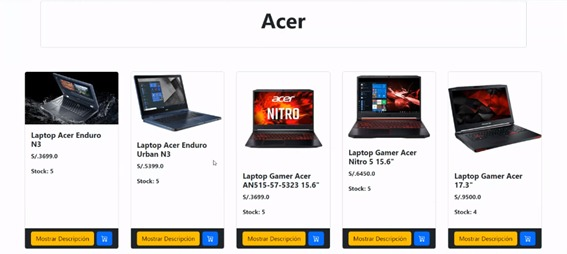
\includegraphics[width=0.8\textwidth,keepaspectratio]{img/a2.jpeg}
		%\includesvg{img/automata.svg}
		%\label{img:mot2}
		\caption{Productos con carritos de compra como opción.}
    \end{figure}
    \begin{figure}[H]
		\centering
        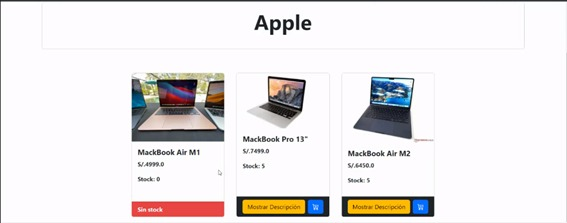
\includegraphics[width=0.8\textwidth,keepaspectratio]{img/a4.jpeg}
		%\includesvg{img/automata.svg}
		%\label{img:mot2}
		\caption{Posible caso de stock de un producto.}
    \end{figure}
    \begin{figure}[H]
		\centering
        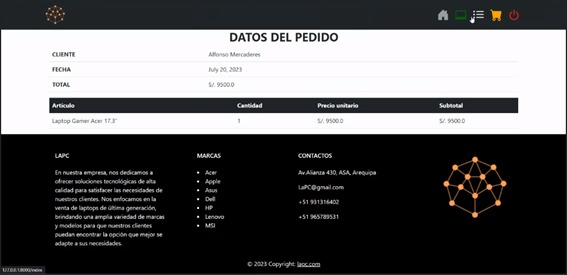
\includegraphics[width=0.8\textwidth,keepaspectratio]{img/a5.jpeg}
		%\includesvg{img/automata.svg}
		%\label{img:mot2}
		\caption{Datos de un pedido.}
    \end{figure}
    \begin{figure}[H]
		\centering
        
\includegraphics[width=0.8\textwidth,keepaspectratio]{img/a6.jpeg}
		%\includesvg{img/automata.svg}
		%\label{img:mot2}
		\caption{Carrito de compras.}
    \end{figure}
    \begin{figure}[H]
		\centering
        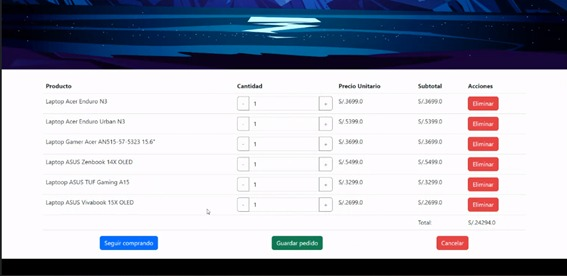
\includegraphics[width=0.8\textwidth,keepaspectratio]{img/a7.jpeg}
		%\includesvg{img/automata.svg}
		%\label{img:mot2}
		\caption{Ejemplo de artículos en el carrito de compras.}
    \end{figure}
    \begin{figure}[H]
		\centering
        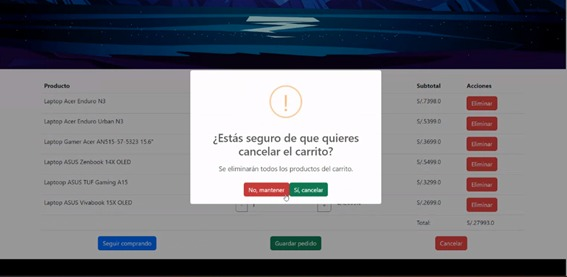
\includegraphics[width=0.8\textwidth,keepaspectratio]{img/a8.jpeg}
		%\includesvg{img/automata.svg}
		%\label{img:mot2}
		\caption{Ejemplo de poder quitar un artículo del carrito de compras.}
    \end{figure}
    \begin{figure}[H]
		\centering
        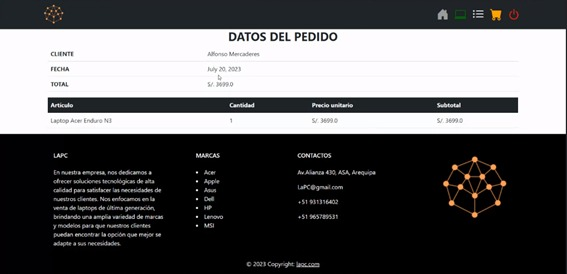
\includegraphics[width=0.8\textwidth,keepaspectratio]{img/a9.jpeg}
		%\includesvg{img/automata.svg}
		%\label{img:mot2}
		\caption{Datos de pedido.}
    \end{figure}


    \begin{figure}[H]
		\centering
        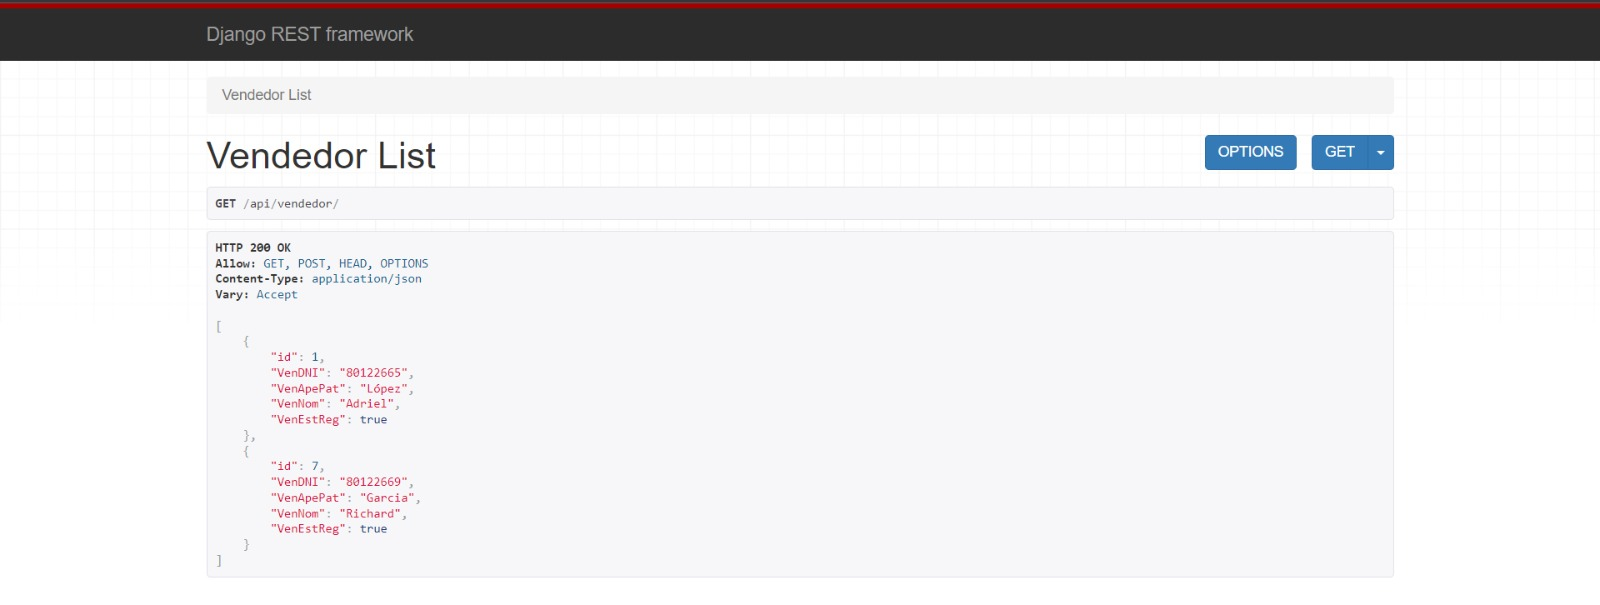
\includegraphics[width=0.8\textwidth,keepaspectratio]{img/b1.jpeg}
		%\includesvg{img/automata.svg}
		%\label{img:mot2}
		\caption{Vendedor List.}
    \end{figure}
    \begin{figure}[H]
		\centering
        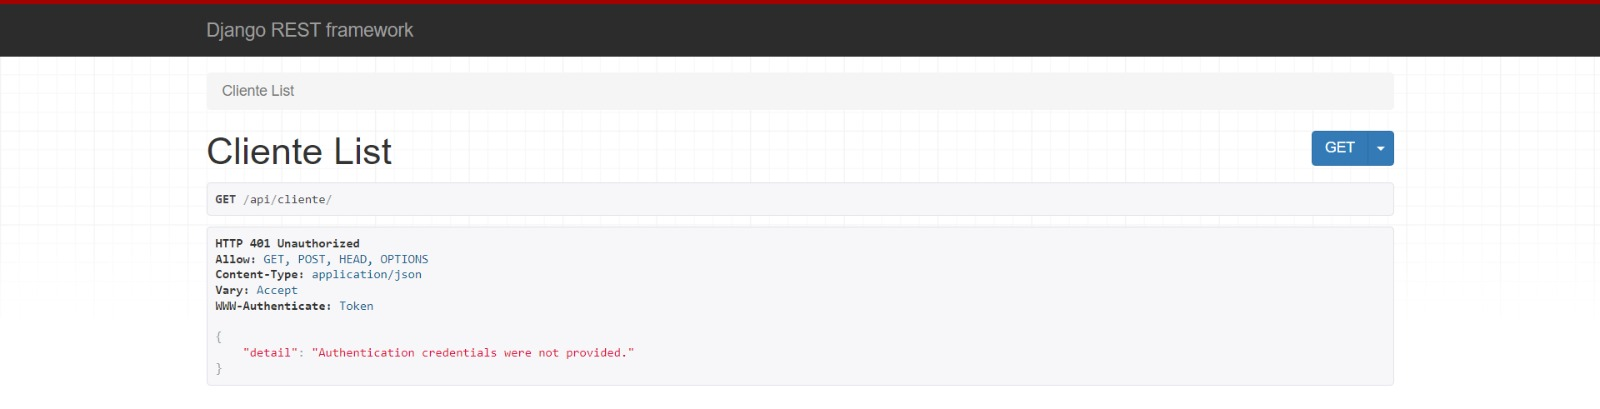
\includegraphics[width=0.8\textwidth,keepaspectratio]{img/b2.jpeg}
		%\includesvg{img/automata.svg}
		%\label{img:mot2}
		\caption{Cliente List.}
    \end{figure}
    \begin{figure}[H]
		\centering
        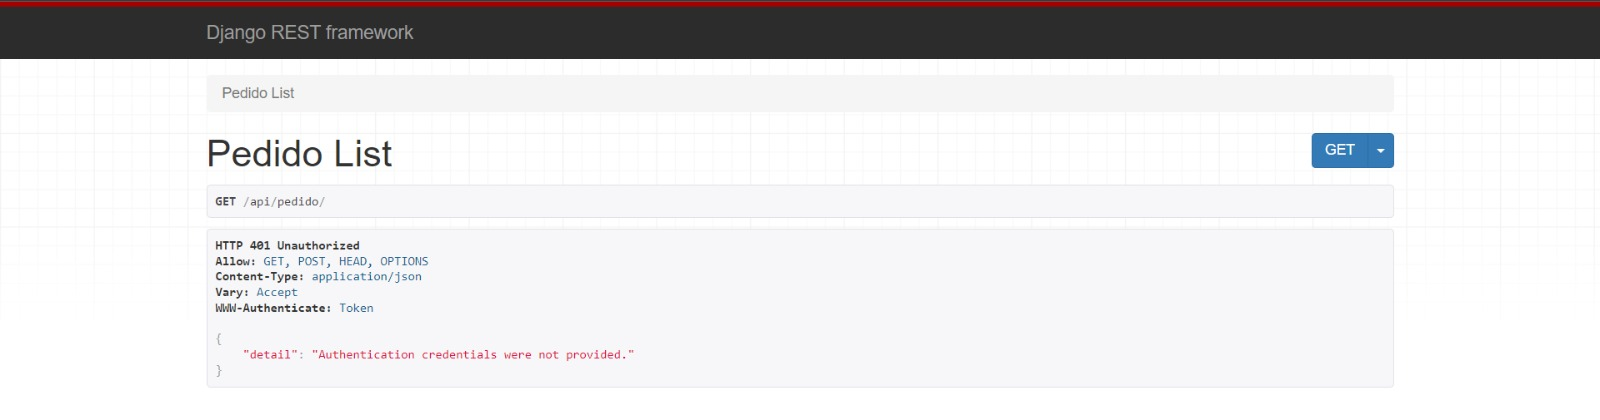
\includegraphics[width=0.8\textwidth,keepaspectratio]{img/b3.jpeg}
		%\includesvg{img/automata.svg}
		%\label{img:mot2}
		\caption{Pedido List.}
    \end{figure}
    \begin{figure}[H]
		\centering
        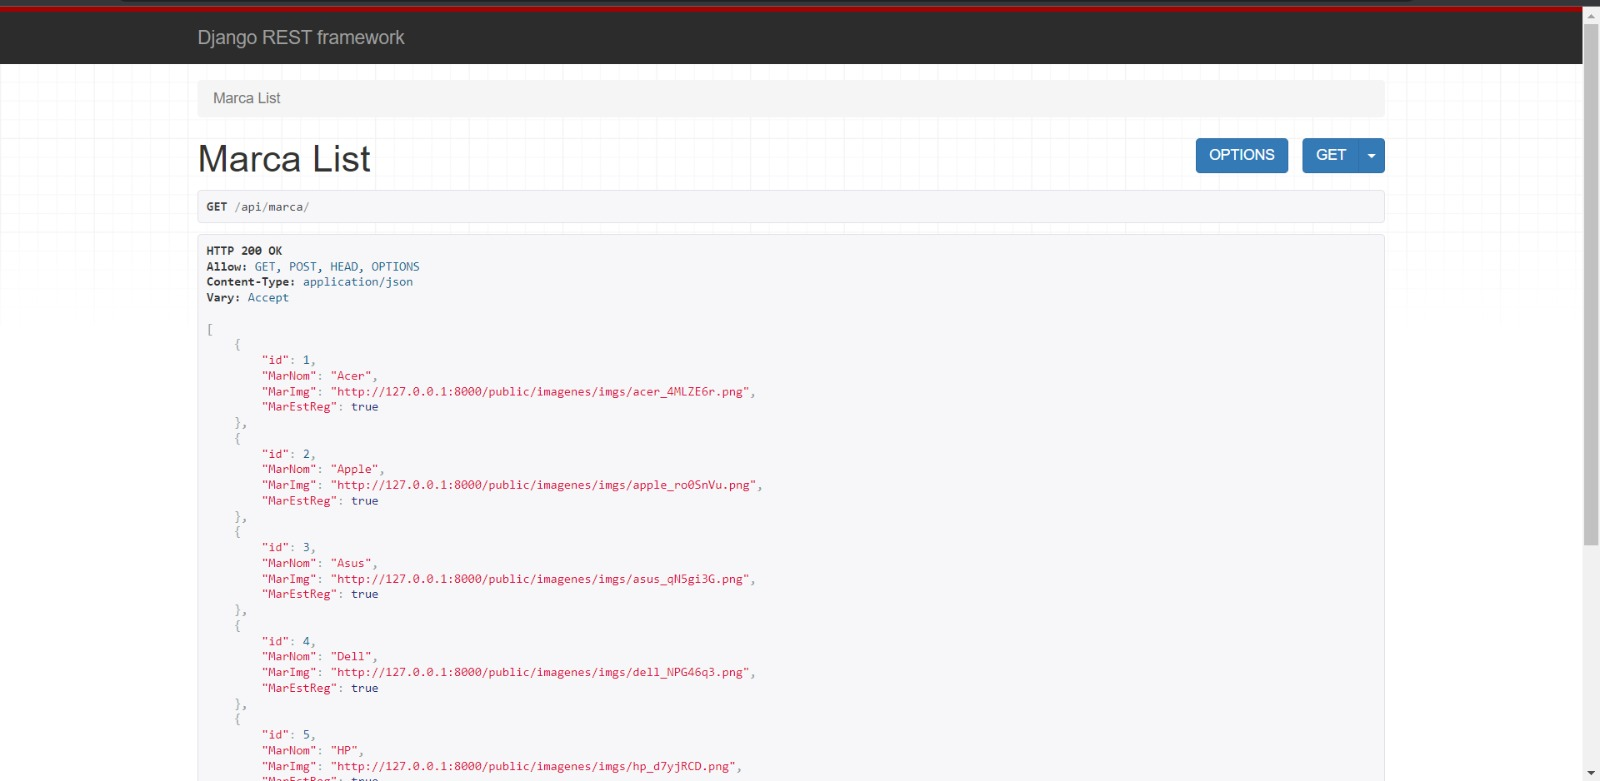
\includegraphics[width=0.8\textwidth,keepaspectratio]{img/b4.jpeg}
		%\includesvg{img/automata.svg}
		%\label{img:mot2}
		\caption{Marca List.}
    \end{figure}
    \begin{figure}[H]
		\centering
        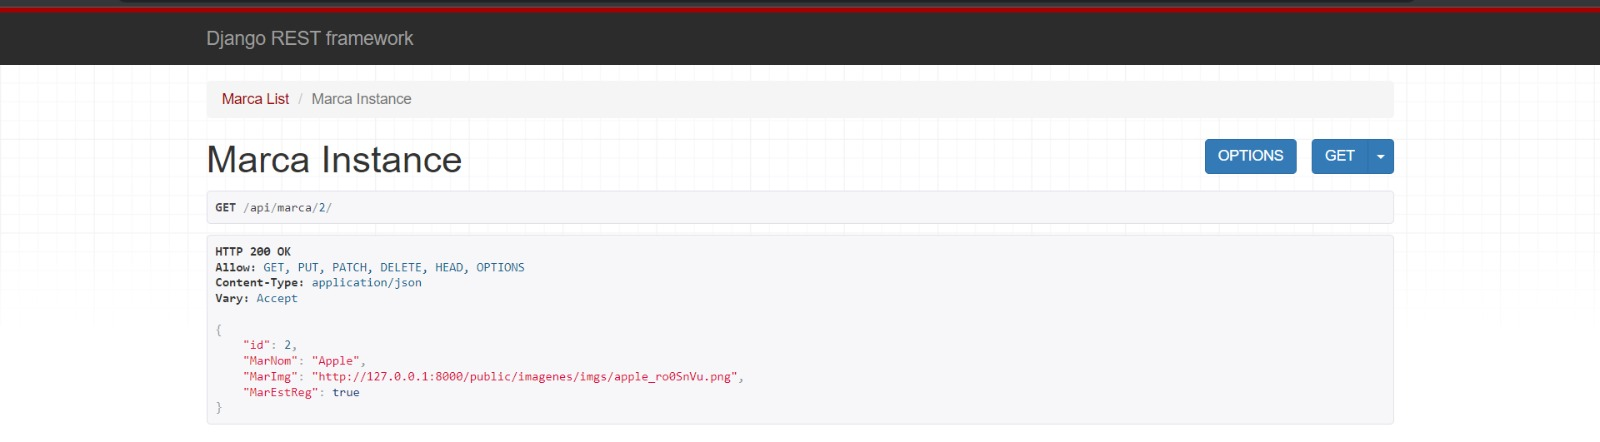
\includegraphics[width=0.8\textwidth,keepaspectratio]{img/b5.jpeg}
		%\includesvg{img/automata.svg}
		%\label{img:mot2}
		\caption{Marca Instance.}
    \end{figure}
    \begin{figure}[H]
		\centering
        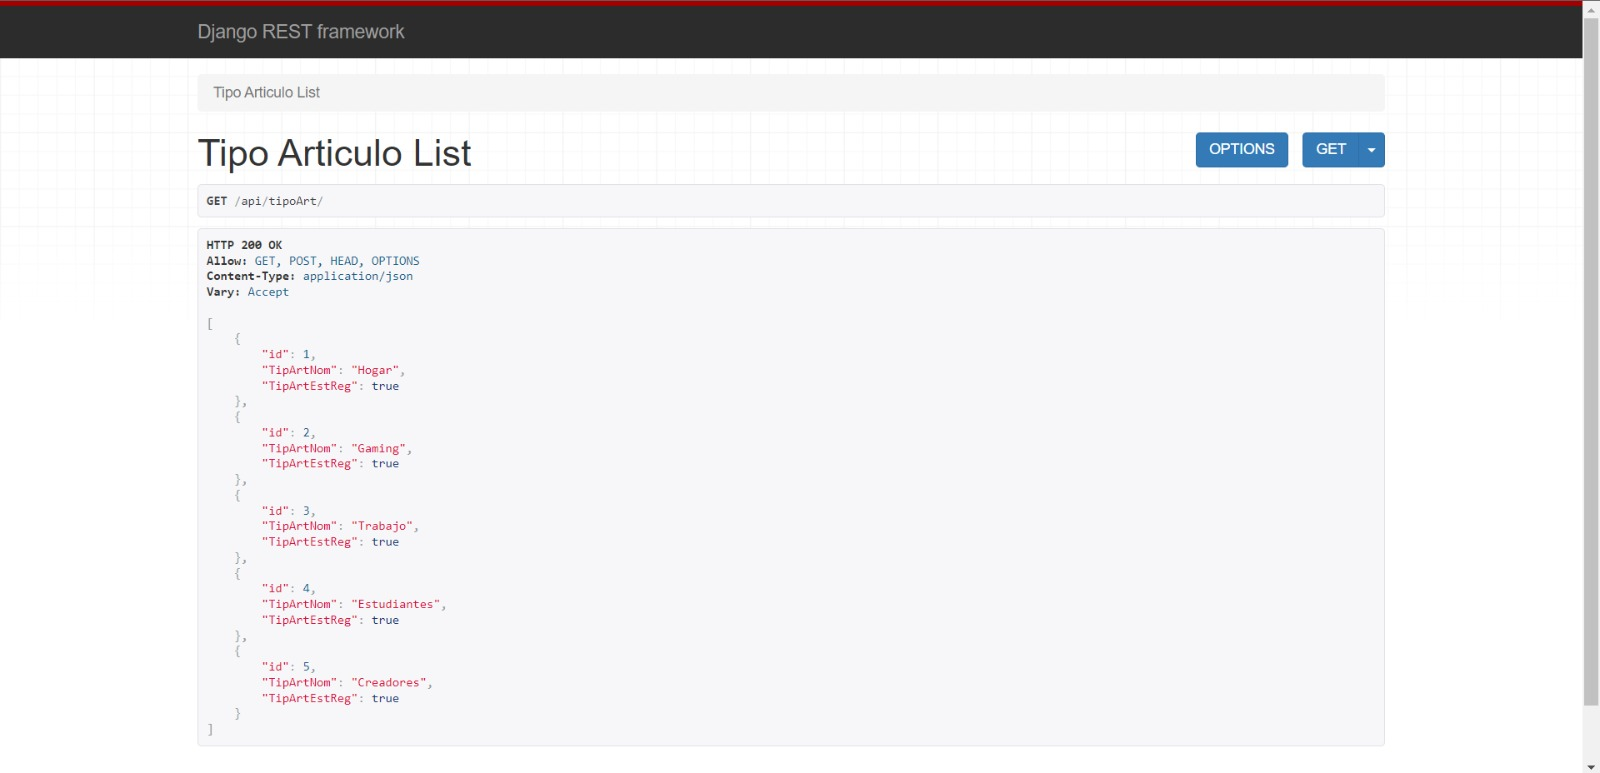
\includegraphics[width=0.8\textwidth,keepaspectratio]{img/b6.jpeg}
		%\includesvg{img/automata.svg}
		%\label{img:mot2}
		\caption{Tipo Artículo List.}
    \end{figure}
    \begin{figure}[H]
		\centering
        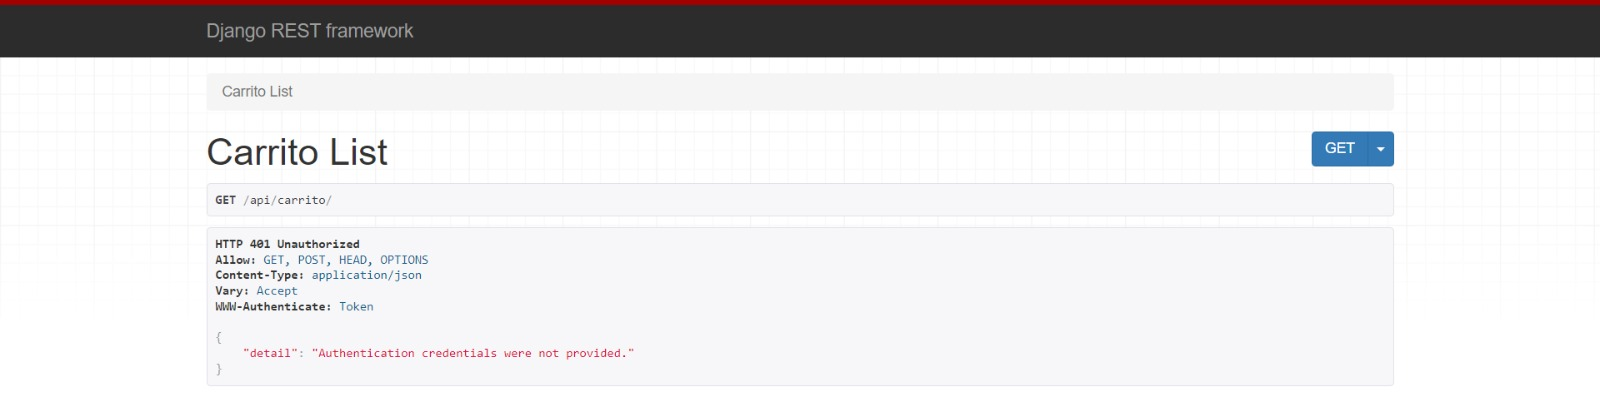
\includegraphics[width=0.8\textwidth,keepaspectratio]{img/b7.jpeg}
		%\includesvg{img/automata.svg}
		%\label{img:mot2}
		\caption{Carrito List.}
    \end{figure}
    \begin{itemize}
        \item Accediento con el token del administrador y usando la extensión de VSC, Thunder Client y GET, vemos la lista de los vendedores actuales. 
    \end{itemize}
    \begin{figure}[H]
		\centering
        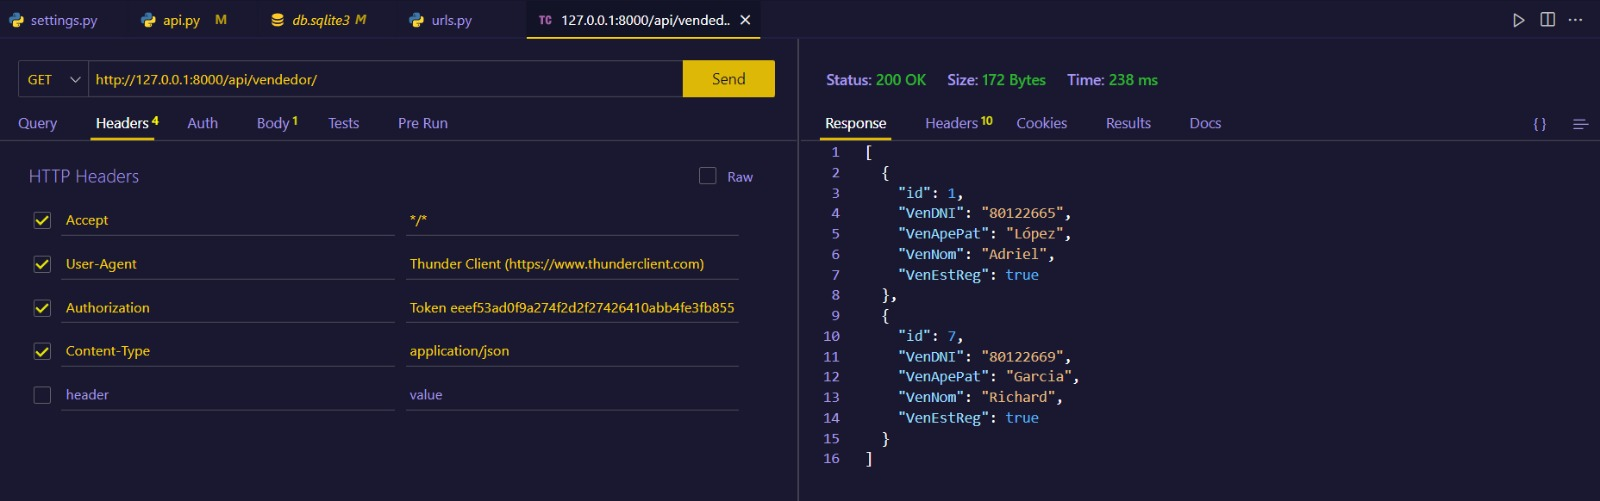
\includegraphics[width=0.8\textwidth,keepaspectratio]{img/b8.jpeg}
		%\includesvg{img/automata.svg}
		%\label{img:mot2}
		\caption{Vendedores.}
    \end{figure}

    \begin{itemize}
        \item Usamos patch para actualizar nombre y ahora se muestra como el vendedor Ronald Garcia está en la lista de Vendedores, tomando el lugar del anterior vendedor Richard.
    \end{itemize}
    \begin{figure}[H]
		\centering
        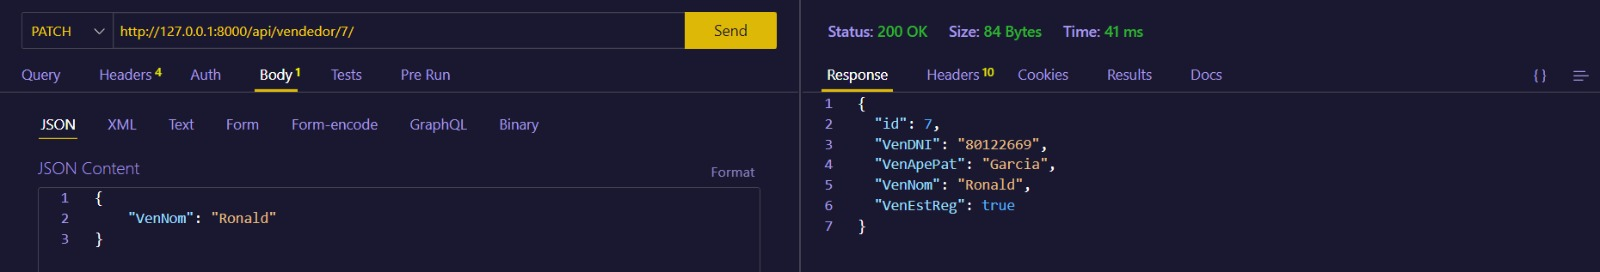
\includegraphics[width=0.8\textwidth,keepaspectratio]{img/b10.jpeg}
		%\includesvg{img/automata.svg}
		%\label{img:mot2}
		\caption{Comprobación de vendedores.}
    \end{figure}
    \begin{itemize}
        \item Ahora eliminaremos al vendedor Ronald usando DELETE.
    \end{itemize}
    \begin{figure}[H]
		\centering
        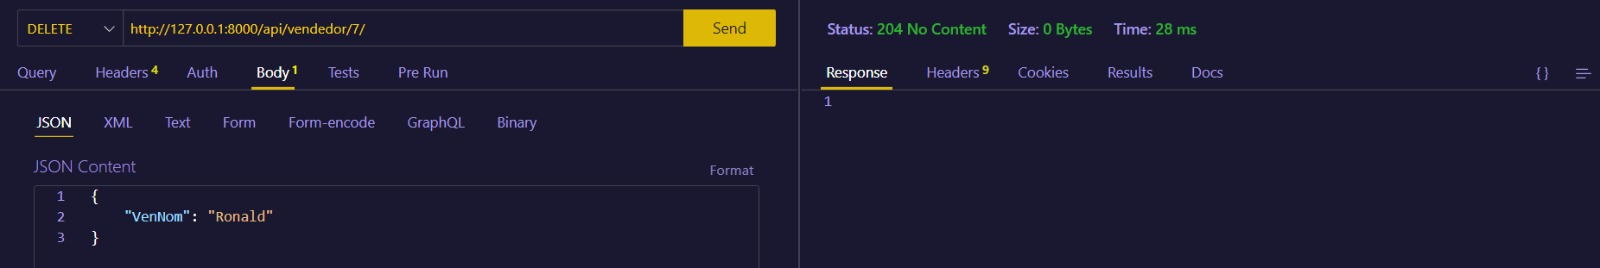
\includegraphics[width=0.8\textwidth,keepaspectratio]{img/b12.jpeg}
		%\includesvg{img/automata.svg}
		%\label{img:mot2}
		\caption{Eliminación de vendedor.}
    \end{figure}
    \begin{itemize}
        \item Ahora creamos auna nueva vendedora llamada Maricielo Gamarra usando POST y  confirmamos que Maricielo está en la lista de vendedores.
    \end{itemize}
  
    \begin{figure}[H]
		\centering
        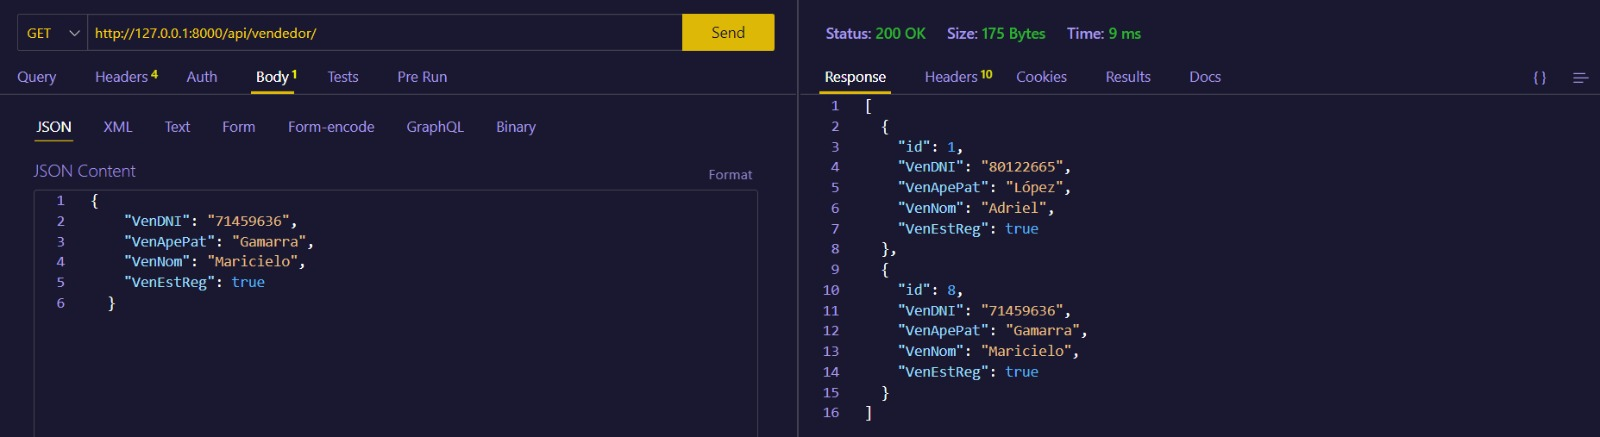
\includegraphics[width=0.8\textwidth,keepaspectratio]{img/b15.jpeg}
		%\includesvg{img/automata.svg}
		%\label{img:mot2}
		\caption{Comprobación de creación de vendedora.}
    \end{figure}
    \begin{itemize}
        \item Ahora veremos los pedidos usando la extensión de Visual Studio Code, Thunder Client.
        \item Se muestra nuestra autorización con el token de admin.
    \end{itemize}
    \begin{figure}[H]
		\centering
        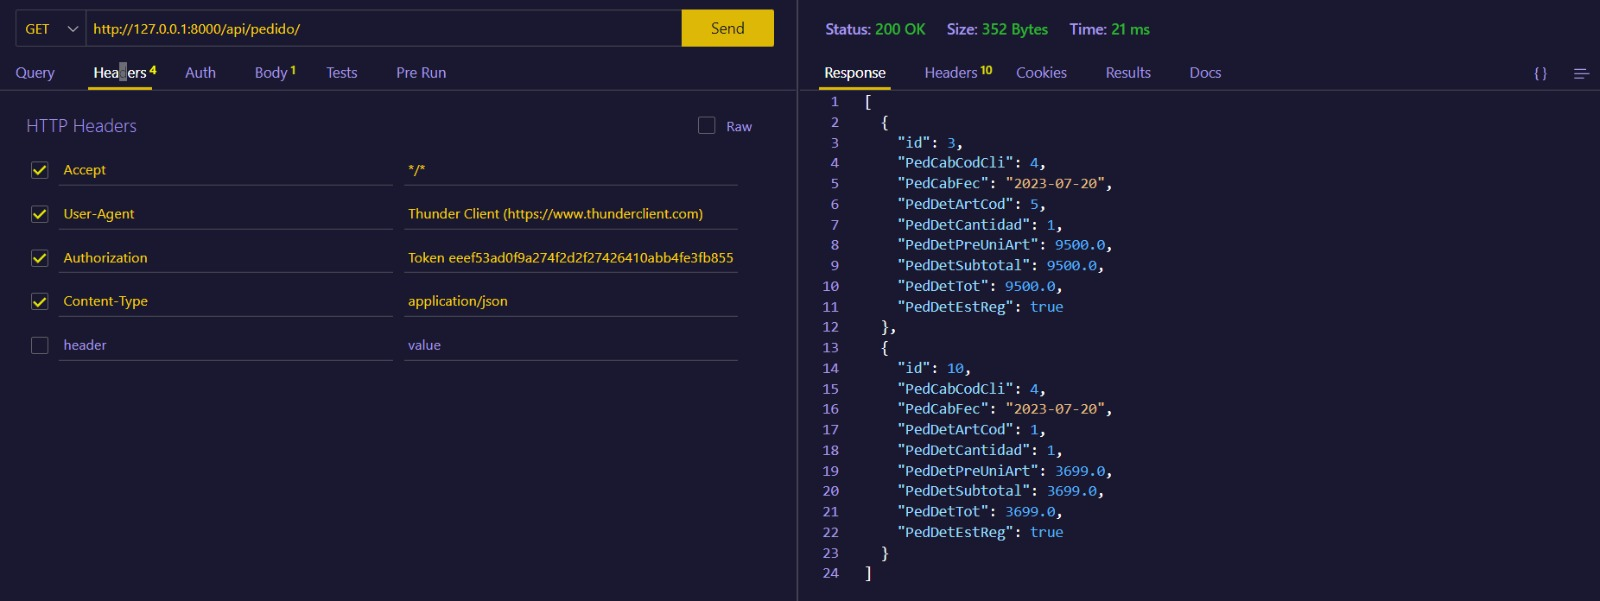
\includegraphics[width=0.8\textwidth,keepaspectratio]{img/b16.jpeg}
		%\includesvg{img/automata.svg}
		%\label{img:mot2}
		\caption{Token admin.}
    \end{figure}
    \begin{itemize}
        \item Se muestra nuestra autorización con el token de Alfonso\_M.
    \end{itemize}
    \begin{figure}[H]
		\centering
        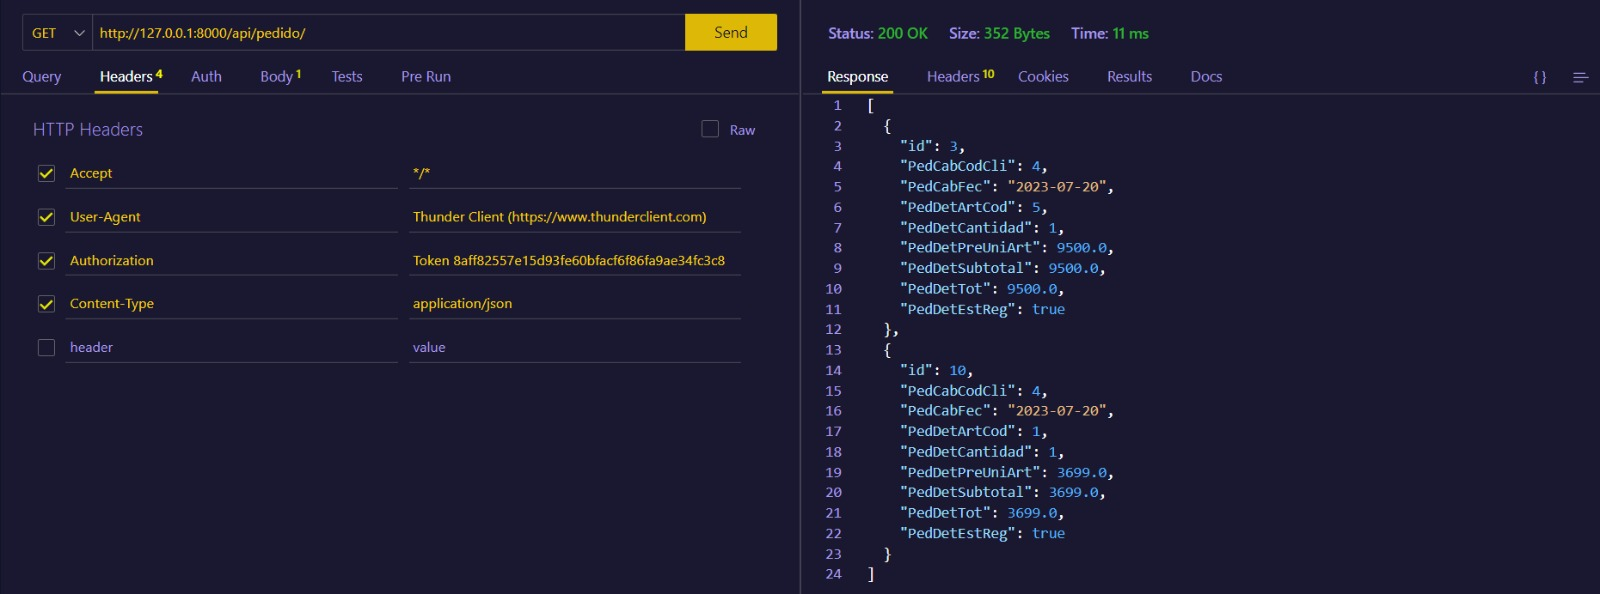
\includegraphics[width=0.8\textwidth,keepaspectratio]{img/b17.jpeg}
		%\includesvg{img/automata.svg}
		%\label{img:mot2}
		\caption{Token Alfonso_M.}
    \end{figure}
    \begin{itemize}
        \item Se muestra cómo es que estamos creando un pedido nuevo.
    \end{itemize}
    \begin{figure}[H]
		\centering
        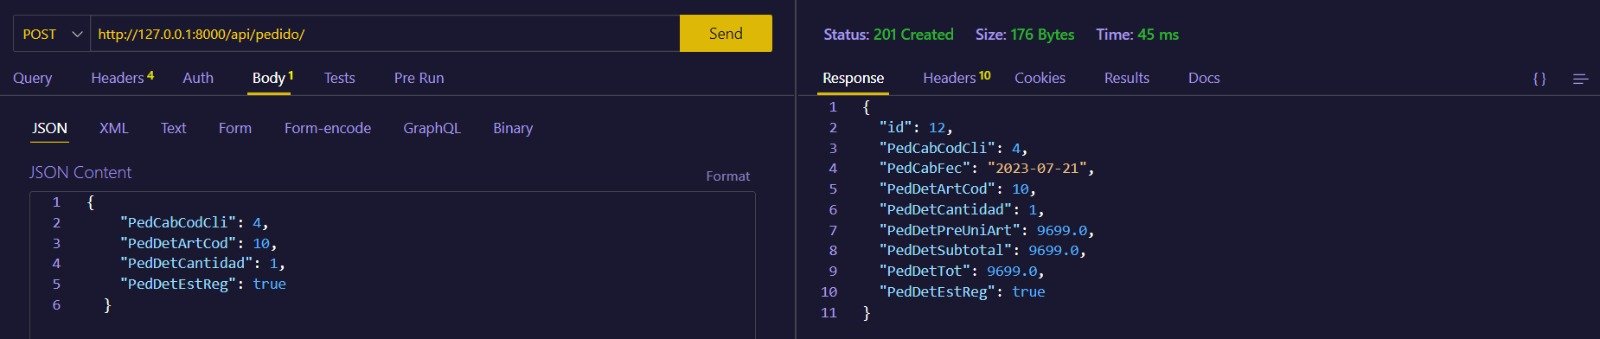
\includegraphics[width=0.8\textwidth,keepaspectratio]{img/b18.jpeg}
		%\includesvg{img/automata.svg}
		%\label{img:mot2}
		\caption{Creación de pedido.}
    \end{figure}
    \begin{itemize}
        \item Se muestra que el pedido ha sido creado.
    \end{itemize}
    \begin{figure}[H]
		\centering
        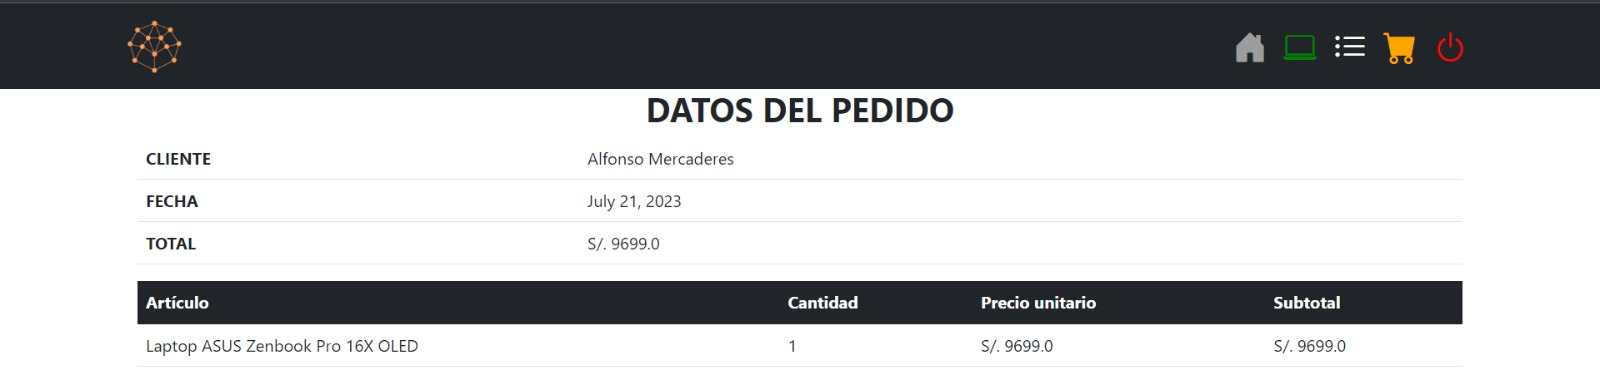
\includegraphics[width=0.8\textwidth,keepaspectratio]{img/b19.jpeg}
		%\includesvg{img/automata.svg}
		%\label{img:mot2}
		\caption{Pedido.}
    \end{figure}
    \begin{itemize}
        \item A continuación se muestra como obtenemos todos los pedidos usando GET.
    \end{itemize}
    \begin{figure}[H]
		\centering
        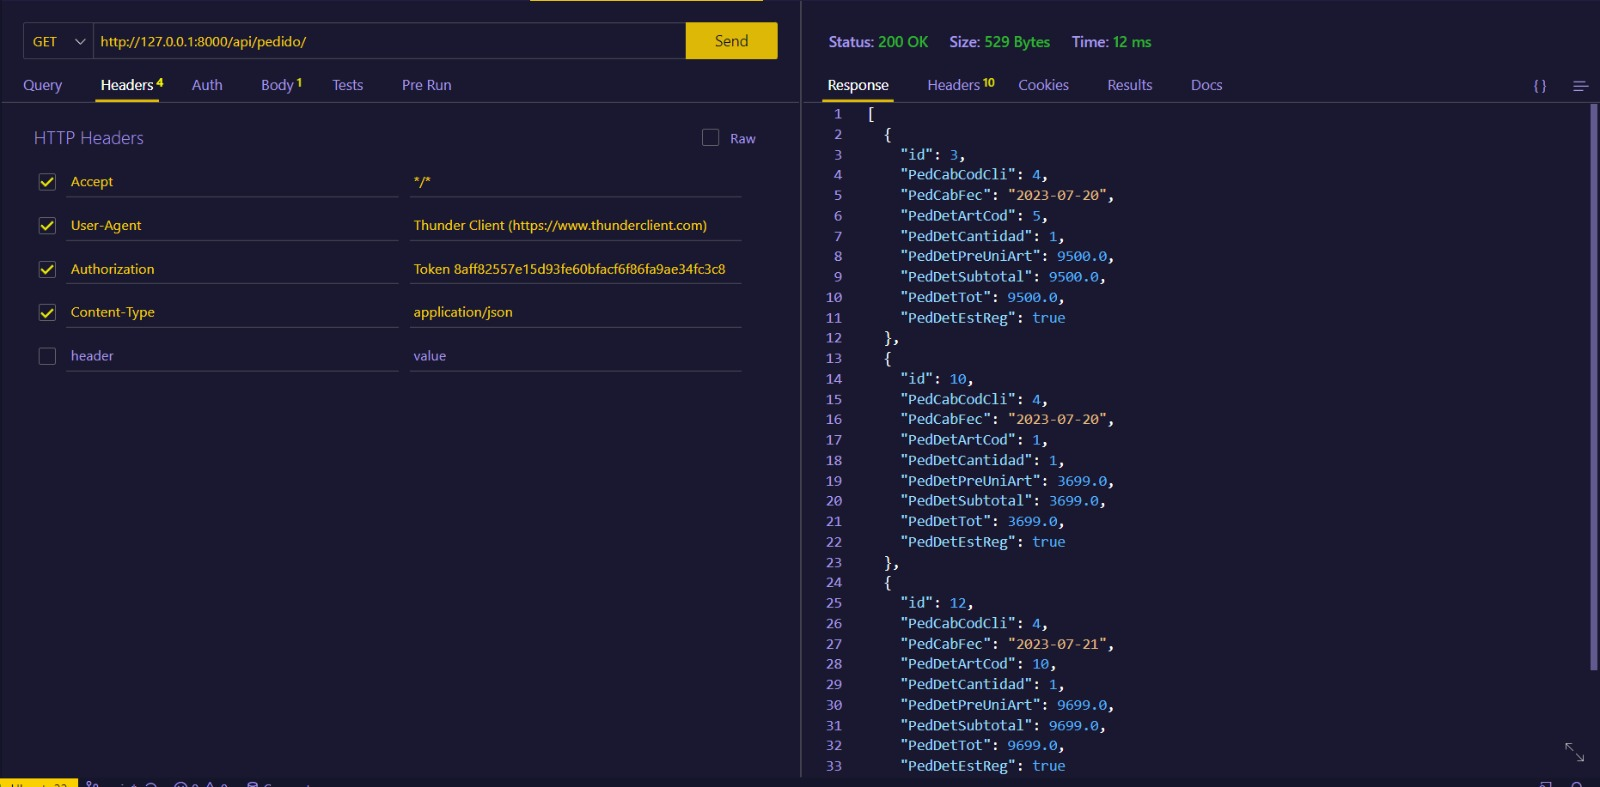
\includegraphics[width=0.8\textwidth,keepaspectratio]{img/b20.jpeg}
		%\includesvg{img/automata.svg}
		%\label{img:mot2}
		\caption{Obtención de pedidos.}
    \end{figure}
    \begin{itemize}
        \item Se muestra cómo se elimina el pedido.
    \end{itemize}
    \begin{figure}[H]
		\centering
        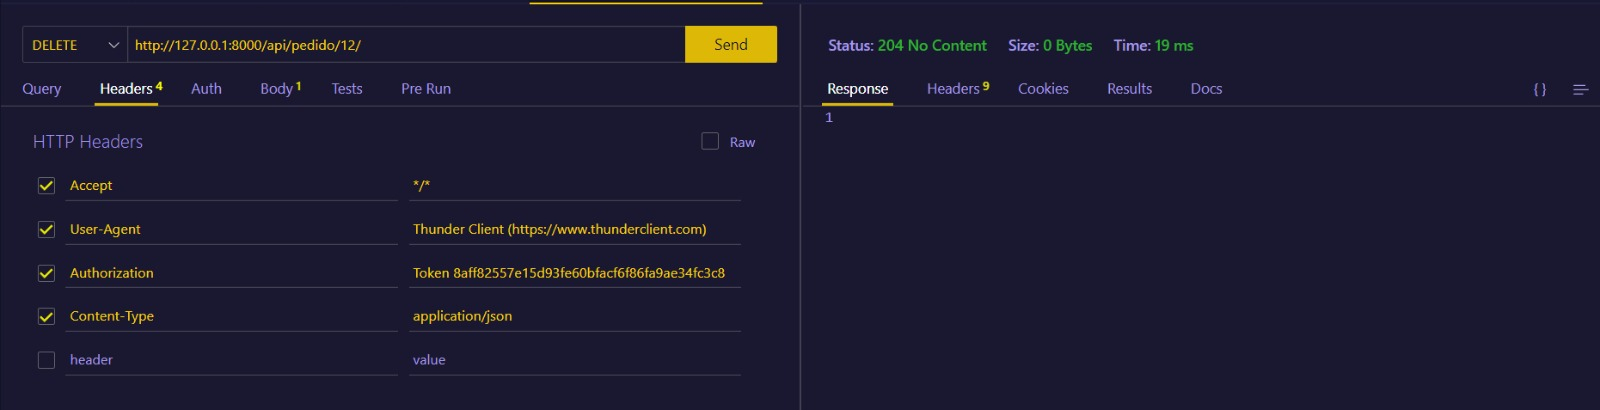
\includegraphics[width=0.8\textwidth,keepaspectratio]{img/b21.jpeg}
		%\includesvg{img/automata.svg}
		%\label{img:mot2}
		\caption{Eliminación de un pedido.}
    \end{figure}
    \begin{itemize}
        \item Ahora comprobamos el estado de nuestro carrito de compras.
    \end{itemize}
    \begin{figure}[H]
		\centering
        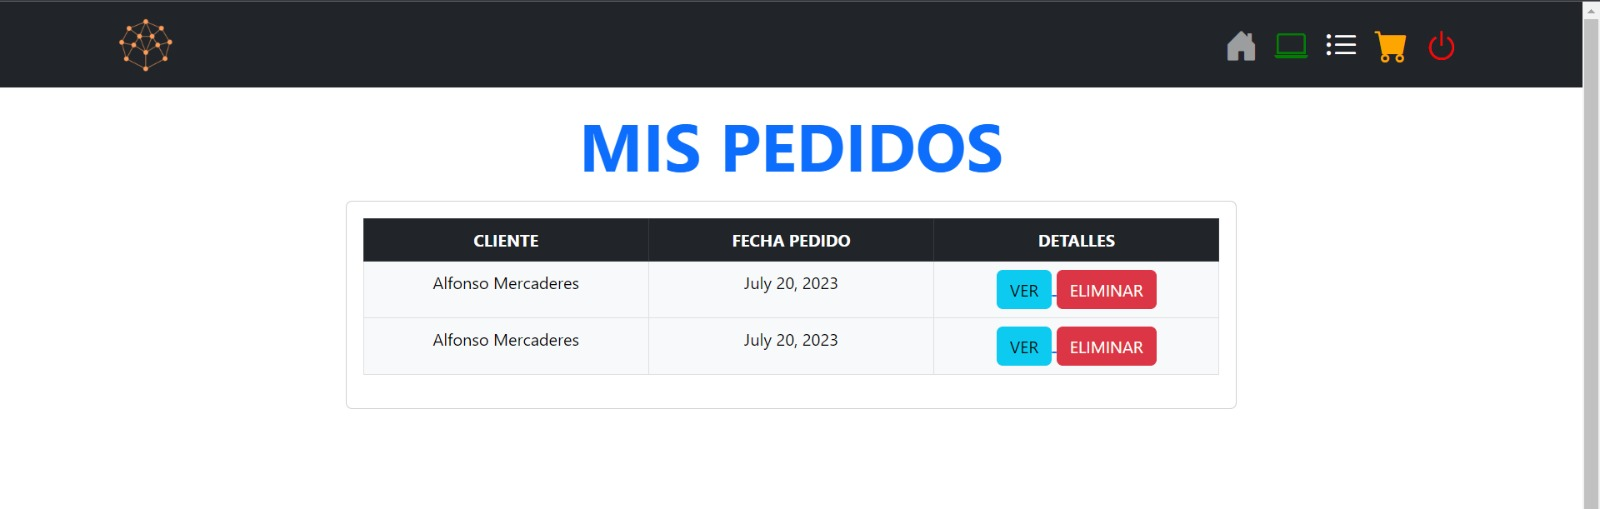
\includegraphics[width=0.8\textwidth,keepaspectratio]{img/b22.jpeg}
		%\includesvg{img/automata.svg}
		%\label{img:mot2}
		\caption{Verificación.}
    \end{figure}
    \begin{itemize}
        \item En la siguiente imágen se muestra la validacón y comprobación.
    \end{itemize}
    \begin{figure}[H]
		\centering
        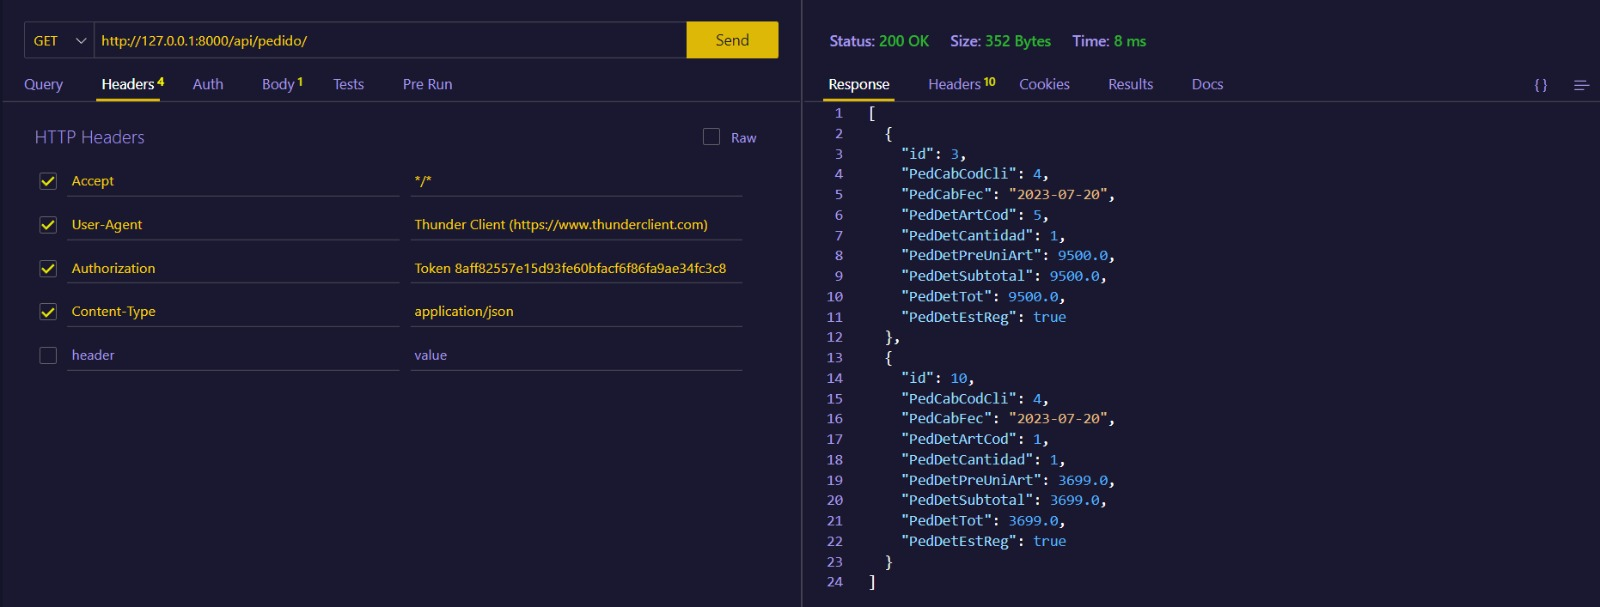
\includegraphics[width=0.8\textwidth,keepaspectratio]{img/b23.jpeg}
		%\includesvg{img/automata.svg}
		%\label{img:mot2}
		\caption{Validación y comprobación.}
    \end{figure}

    \section{Commits}
    \begin{itemize}
        \item Funcionalidad carrito de compras funcional, se realizó la comprobación de la eficacia del carrito de compras.
        \item Redireccionamiento signin, singup, esto cuando no se halla creado una cuenta previamente.
        \item Función de Token para cada usuario, se hizo para que cada usuarioi logre ver sus pedidos.
        \item Los commits son los siguientes:
    \end{itemize}
    \begin{figure}[H]
		      \centering
                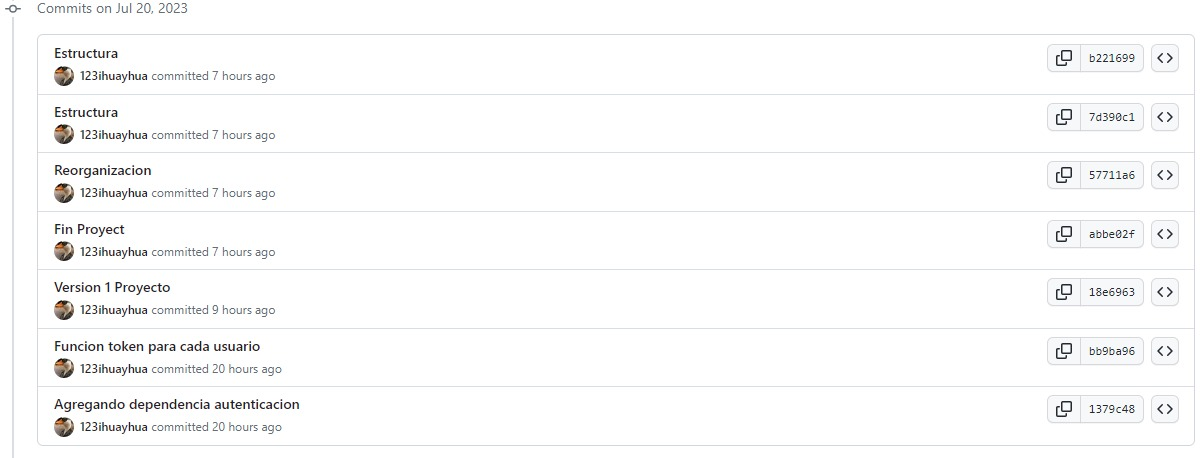
\includegraphics[width=0.8\textwidth,keepaspectratio]{img/c1.jpeg}
		      %\includesvg{img/automata.svg}
		      %\label{img:mot2}
		      %\caption{Product backlog.}
	   \end{figure}
    \begin{figure}[H]
		      \centering
                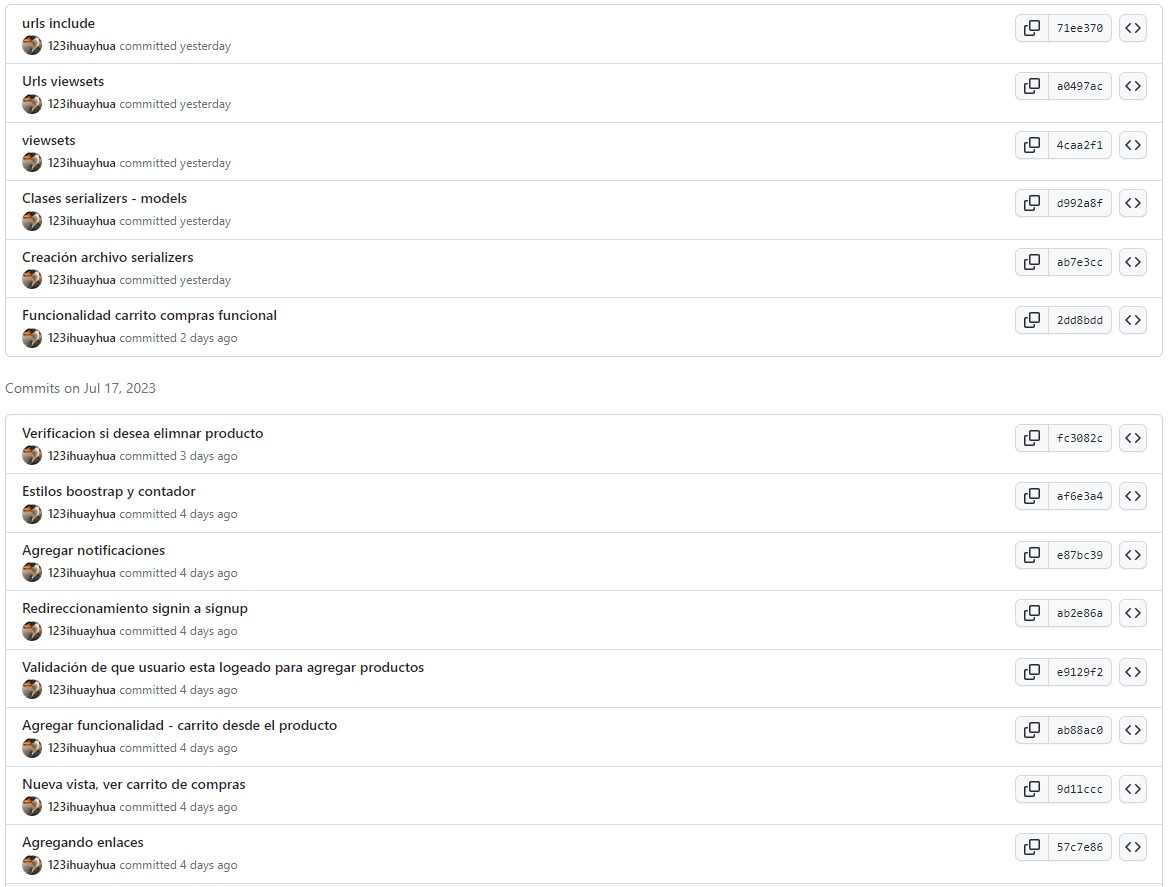
\includegraphics[width=0.8\textwidth,keepaspectratio]{img/c2.jpeg}
		      %\includesvg{img/automata.svg}
		      %\label{img:mot2}
		      %\caption{Product backlog.}
	   \end{figure}
    \begin{figure}[H]
		      \centering
                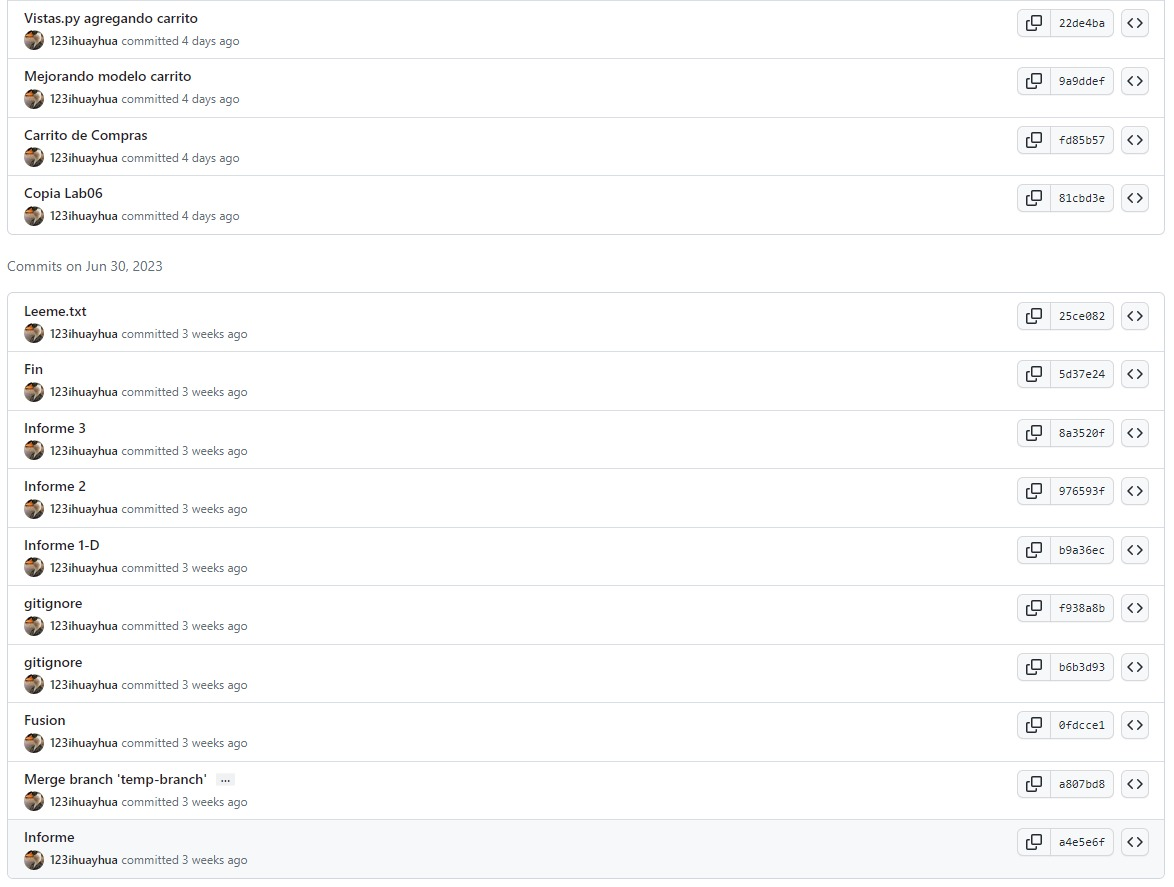
\includegraphics[width=0.8\textwidth,keepaspectratio]{img/c3.jpeg}
		      %\includesvg{img/automata.svg}
		      %\label{img:mot2}
		      %\caption{Product backlog.}
	   \end{figure}

    


		

	\section{\textcolor{red}{Rúbricas}}
	
	\subsection{\textcolor{red}{Entregable Informe}}
	\begin{table}[H]
		\caption{Tipo de Informe}
		\setlength{\tabcolsep}{0.5em} % for the horizontal padding
		{\renewcommand{\arraystretch}{1.5}% for the vertical padding
		\begin{tabular}{|p{3cm}|p{12cm}|}
			\hline
			\multicolumn{2}{|c|}{\textbf{\textcolor{red}{Informe}}}  \\
			\hline 
			\textbf{\textcolor{red}{Latex}} & \textcolor{blue}{El informe está en formato PDF desde Latex,  con un formato limpio (buena presentación) y facil de leer.}   \\ 
			\hline 
			
			
		\end{tabular}
	}
	\end{table}
	
	\clearpage
	
	\subsection{\textcolor{red}{Rúbrica para el contenido del Informe y demostración}}
	\begin{itemize}			
		\item El alumno debe marcar o dejar en blanco en celdas de la columna \textbf{Checklist} si cumplio con el ítem correspondiente.
		\item Si un alumno supera la fecha de entrega,  su calificación será sobre la nota mínima aprobada, siempre y cuando cumpla con todos lo items.
		\item El alumno debe autocalificarse en la columna \textbf{Estudiante} de acuerdo a la siguiente tabla:
	
		\begin{table}[ht]
			\caption{Niveles de desempeño}
			\begin{center}
			\begin{tabular}{ccccc}
    			\hline
    			 & \multicolumn{4}{c}{Nivel}\\
    			\cline{1-5}
    			\textbf{Puntos} & Insatisfactorio 25\%& En Proceso 50\% & Satisfactorio 75\% & Sobresaliente 100\%\\
    			\textbf{2.0}&0.5&1.0&1.5&2.0\\
    			\textbf{4.0}&1.0&2.0&3.0&4.0\\
    		\hline
			\end{tabular}
		\end{center}
	\end{table}	
	
	\end{itemize}
	
	\begin{table}[H]
		\caption{Rúbrica para contenido del Informe y demostración}
		\setlength{\tabcolsep}{0.5em} % for the horizontal padding
		{\renewcommand{\arraystretch}{1.5}% for the vertical padding
		%\begin{center}
		\begin{tabular}{|p{2.7cm}|p{7cm}|x{1.3cm}|p{1.2cm}|p{1.5cm}|p{1.1cm}|}
			\hline
    		\multicolumn{2}{|c|}{Contenido y demostración} & Puntos & Checklist & Estudiante & Profesor\\
			\hline
			\textbf{1. GitHub} & Hay enlace URL activo del directorio para el  laboratorio hacia su repositorio GitHub con código fuente terminado y fácil de revisar. &2 &X &2 & \\ 
			\hline
			\textbf{2. Commits} &  Hay capturas de pantalla de los commits más importantes con sus explicaciones detalladas. (El profesor puede preguntar para refrendar calificación). &4 &X &4 & \\ 
			\hline 
			\textbf{3. Código fuente} &  Hay porciones de código fuente importantes con numeración y explicaciones detalladas de sus funciones. &2 &X &2 & \\ 
			\hline 
			\textbf{4. Ejecución} & Se incluyen ejecuciones/pruebas del código fuente  explicadas gradualmente. &2 &X &1 & \\ 
			\hline			
			\textbf{5. Pregunta} & Se responde con completitud a la pregunta formulada en la tarea.  (El profesor puede preguntar para refrendar calificación).  &2 &X &1 & \\ 
			\hline	
			\textbf{6. Fechas} & Las fechas de modificación del código fuente estan dentro de los plazos de fecha de entrega establecidos. &2 &X &2 & \\ 
			\hline 
			\textbf{7. Ortografía} & El documento no muestra errores ortográficos. &2 &X &2 & \\ 
			\hline 
			\textbf{8. Madurez} & El Informe muestra de manera general una evolución de la madurez del código fuente,  explicaciones puntuales pero precisas y un acabado impecable.   (El profesor puede preguntar para refrendar calificación).  &4 &X &3 & \\ 
			\hline
			\multicolumn{2}{|c|}{\textbf{Total}} &20 & &17 & \\ 
			\hline
		\end{tabular}
		%\end{center}
		%\label{tab:multicol}
		}
	\end{table}
	
\clearpage

\section{Referencias}
\begin{itemize}			
    \item {https://developer.mozilla.org/en-US/docs/Learn/Server-side/Django/Tutorial_local_
library_website}
    \item \url{https://github.com/mdn/django-locallibrary-tutorial}
    \item \url{https://github.com/rescobedoq/pw2/tree/main/labs/lab05}
    \item William S. Vincent. (2022). Django for Beginners: Build websites with Python. Django 4.0.
leanpub.com. [URL]
    \item \url{https://docs.djangoproject.com/en/4.1/ref/models/fields/}
    \item \url{https://docs.djangoproject.com/en/4.0/topics/db/examples/many_to_many/}
    \item \url{https://docs.djangoproject.com/en/4.0/topics/db/examples/many_to_one/}
    \item \url{https://blog.hackajob.co/djangos-new-database-constraints/}
    \item \url{https://stackoverflow.com/questions/3330435/is-there-an-sqlite-equivalent-to-mysqls-describe-table}
    \item \url{https://docs.djangoproject.com/en/4.1/ref/validators/#how-validators-are-run}
    \item \url{https://docs.djangoproject.com/en/4.1/ref/models/instances/}
    \item \url{https://www.youtube.com/watch?v=rHux0gMZ3Eg}
    \item \url{https://www.youtube.com/watch?v=OTmQOjsl0eg}
    \item \url{https://tex.stackexchange.com/questions/34580/escape-character-in-latex}
    \item \url{https://www.sqlitetutorial.net/sqlite-show-tables/}
    \item \url{https://www.wplogout.com/export-database-diagrams-erd-from-django/}
\end{itemize}	
	
%\clearpage
%\bibliographystyle{apalike}
%\bibliographystyle{IEEEtranN}
%\bibliography{bibliography}
			
\end{document}